\section{The numbers of \protein{BubR1}, \protein{Bub1}, and \protein{Mad1} recruited per signaling kinetochore are inversely correlated with the total number of signaling kinetochores in the cell}

To evaluate how the number of \protein{BubR1}, \protein{Bub1}, and \protein{Mad1} proteins recruited per signaling kinetochore changes with the total number of signaling kinetochores in the cell, We first need to obtain mitotic cells containing distinctly different numbers of signaling kinetochores.

To obtain mitotic cells with nearly all kinetochores activating the SAC, we released G\textsubscript{1}/S-arrested cells and then treated them with \SI{330}{nM} nocodazole, a drug that destabilizes microtubules. These nocodazole-treated cells resemble normal mitotic cells at the start of the prometaphase.

To obtain mitotic cells with a much smaller number of signaling kinetochores, we released G\textsubscript{1}/S-arrested cells and then treated them with GSK923295, a \protein{Cenp-E} inhibitor \cite{GSK923295}. In these cells, usually a variable but smaller number of chromosomes are stranded near the spindle poles (\myref{SACProteinKinetochoreRecruitment_Images}). We analyzed only those cells that contained ten or less than ten polar chromosomes. Kinetochores on these polar chromosomes are either unattached or laterally attached, which activate the SAC \cite{GSK923295LateralAttachmentEM, GSK923295MonastrolCotreatment}. These GSK923295-treated cells arguably (see discussions in \myref{Chapter3Discussions}) resemble normal mitotic cells near the end of the prometaphase.

\begin{figure}
    \centering
    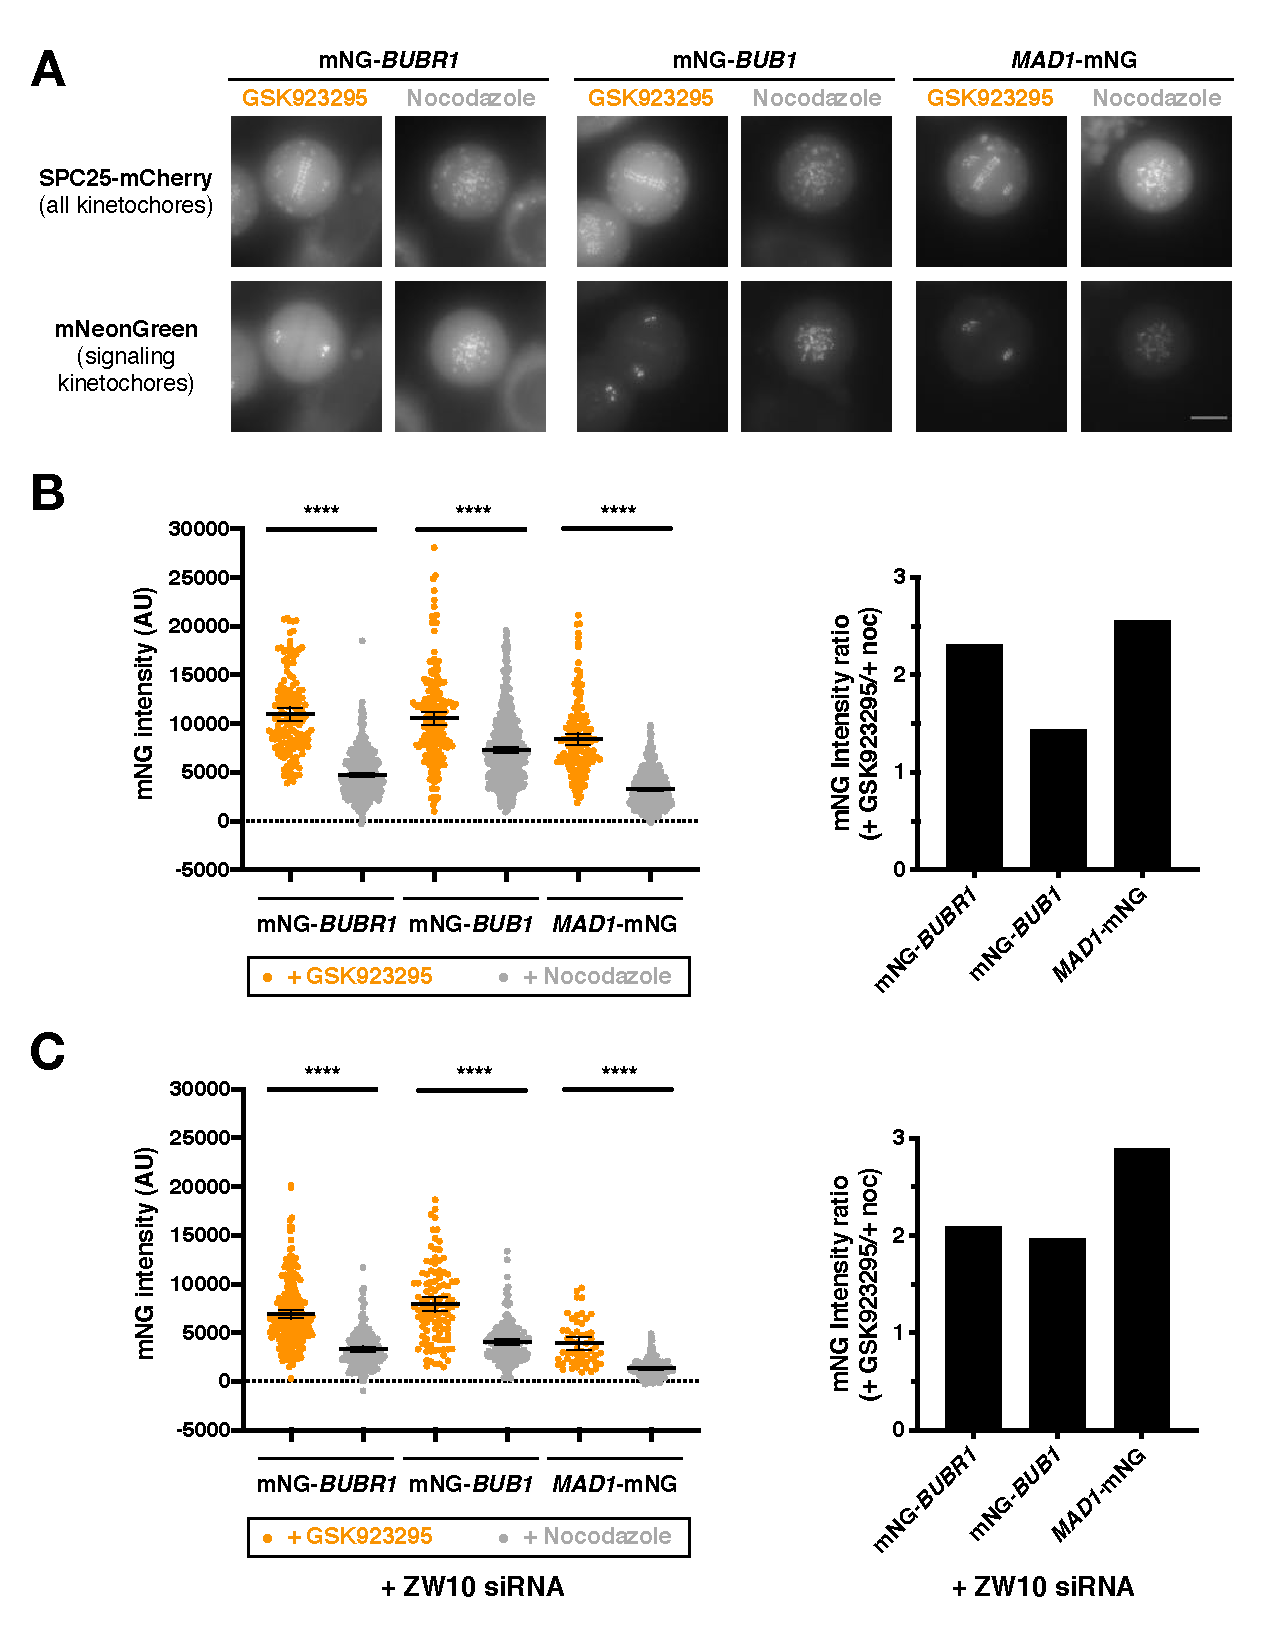
\includegraphics[width=\textwidth]{chapters/figures/SACProteinKinetochoreRecruitment.pdf}
    \phantomsubfiglabel{SACProteinKinetochoreRecruitment_Images} % subfigure A
    \phantomsubfiglabel{SACProteinKinetochoreRecruitment_Quantification} % subfigure B
    \phantomsubfiglabel{siZW10SACProteinKinetochoreRecruitment_Quantification} % subfigure C
    \caption{The numbers of \protein{BubR1}, \protein{Bub1}, and \protein{Mad1} recruited per signaling kinetochore are inversely correlated with the total number of signaling kinetochores in the cell.}}
    \noindent\justifying \myref{SACProteinKinetochoreRecruitment_Quantification,siZW10SACProteinKinetochoreRecruitment_Quantification} were reproduced from one of my first-author manuscripts in preparation. Lauren Humphrey-Stark performed all imaging experiments and data analysis involved in this figure. (A) Exemplary micrographs showing cells from the three HeLa-A12 cell lines treated with nocodazole or GSK923295. Spc25-mCherry labeled all kinetochores. Scale bar, \SI{10}{\micro m}. (B) Left panel: quantification of mNeonGreen signals at individual signaling kinetochores from experiments illustrated in (A). Each dot represents the measurement from one signaling kinetochore. Error bars represent 95\% confidence intervals of the mean. Results from at least two independent experiments are shown. Right panel: Pairwise ratios between the average mNeonGreen signals at individual signaling kinetochores of GSK923295-treated cells and nocodazole-treated cells in the left panel. (C) Similar to (B), except that all cells were additionally treated with a siRNA against \gene{ZW10}.
    % Bub1/BubR1 recruitment data with knockdown of the RZZ complex compared with those with no siRNA deviate greatly from Zhang et al., 2019
\label{SACProteinKinetochoreRecruitment}
\end{figure}

In nocodazole-treated cells, the number of mNG-\protein{BubR1} and \protein{Mad1}-mNG proteins recruited per signaling kinetochore in nocodazole-treated cells was lower than that of mNG-\protein{Bub1} recruitment (\myref{SACProteinKinetochoreRecruitment_Quantification}). Importantly, \protein{BubR1}, \protein{Bub1}, and \protein{Mad1} recruitment per signaling kinetochore were all significantly increased when cells were treated with GSK923295 compared to nocodazole (\myref{SACProteinKinetochoreRecruitment_Quantification}). This confirms that the number of SAC proteins recruited per kinetochore is indeed inversely correlated with the number of signaling kinetochores in the cell.%This is consistent with observations made in budding yeast (Aravamudhan et al., 2016).

\protein{Mad1} is also recruited to the fibrous coronae around metazoan kinetochores, which contribute to the measurement in \myref{SACProteinKinetochoreRecruitment_Quantification}. The fibrous coronae constituents \protein{Cenp-E} and \protein{Cenp-F} interact with \protein{BubR1} and \protein{Bub1}, respectively \cite{CENPELocalization-BUBR1, CENP-FLimitsStripping}. %cyclin B1 references (Pereira et al., 2018; Rodriguez-Rodriguez et al., 2018; Silio et al., 2015)
To dissect how much the core SAC signaling cascade contributes to the recruitment of these SAC proteins at signaling kinetochores, we knocked down \gene{ZW10}, a subunit of the RZZ complex, by treating the genome-edited HeLa-A12 cells with a siRNA against \gene{ZW10}. We then quantified the recruitment of the mNG-labeled SAC proteins to signaling kinetochores as before. As expected, \protein{Mad1} recruitment was significantly lower in both GSK923295 and nocodazole-treated cells (\myref{siZW10SACProteinKinetochoreRecruitment_Quantification}). The number of \protein{Mad1} molecules recruited was reduced approximately by half, revealing the contribution of the RZZ under these conditions. The number of \protein{BubR1} and \protein{Bub1} molecules recruited per signaling kinetochore was also reduced. % as noted by others (Kops et al., 2005).
Importantly, the number of SAC proteins recruited per kinetochore is still inversely correlated with the number of signaling kinetochores in the cell.